\documentclass[a4paper,14pt]{extarticle}

\usepackage[T2A]{fontenc}			
\usepackage[utf8]{inputenc}			
\usepackage[english,russian]{babel}

\usepackage[
bookmarks=true, colorlinks=true, unicode=true,
urlcolor=black,linkcolor=black, anchorcolor=black,
citecolor=black, menucolor=black, filecolor=black,
]{hyperref}

\usepackage{color}
\usepackage{caption}
\DeclareCaptionFont{white}{\color{black}}
\DeclareCaptionFormat{listing}{\colorbox{white}{\parbox{\textwidth}{#1#2#3}}}
\captionsetup[lstlisting]{format=listing,labelfont=white,textfont=white}

\usepackage{amsmath,amsfonts,amssymb,amsthm,mathtools} 
\usepackage{wasysym}

%\usepackage[cache=false]{minted}

\usepackage{graphicx}
\usepackage{cmap}
\usepackage{indentfirst}

\usepackage{longtable}

\usepackage{listings} 
\usepackage{fancyvrb}

\usepackage{geometry}
\geometry{left=2cm}
\geometry{right=1.5cm}
\geometry{top=1cm}
\geometry{bottom=2cm}

\setlength{\parindent}{5ex}
\setlength{\parskip}{0.5em}

\usepackage{color}
\usepackage[cache=false, newfloat]{minted}
\newenvironment{code}{\captionsetup{type=listing}}{}
\SetupFloatingEnvironment{listing}{name=Листинг}
 
 
 \begin{document}
 	
 	\def\figurename{Рисунок}
 	
 	\begin{minipage}{0.2\textwidth}
 		
\includegraphics[scale=0.05]{img/bmstu.png}
 	\end{minipage}
 	\begin{minipage}{0.7\textwidth}
 		\small
 		\begin{center}
 			\textbf{Министерство науки и высшего образования Российской Федерации}
 			
 			\textbf{Федеральное государственное бюджетное образовательное учреждение высшего образования «Московский государственный технический университет имени Н.Э. Баумана}
 			
 			\textbf{(национальный исследовательский университет)»}
 			
 			\textbf{(МГТУ им. Н.Э. Баумана)}
 		\end{center}
 	\end{minipage}
 	
 	\vspace*{5mm}
 	
 	\normalsize
 	\begin{flushleft}
 		Факультет: <<Информатика и системы управления>>
 		
 		Кафедра: <<Программное обеспечение ЭВМ и информационные технологии>>
 	\end{flushleft}
 	
 	\vspace*{30mm}
 	
 	\LARGE
 	\begin{center}
 		\textbf{Расчетно-пояснительная записка}
 		
 		%	\textbf{к курсовому проекту на тему:}
 		\textbf{к курсовой работе на тему:}
 		
 		\textbf{<<Планирование задач в ядре Linux>>}
 	\end{center}
 	
 	\vspace*{15mm}
 	
 	\large
 	\begin{flushleft}
 		\textbf{Студент:} Левушкин И. К. \\
 		\textbf{Группа:} ИУ7-72Б \\
 		%        \textbf{Оценка (баллы):} \\
 		\textbf{Научный руководитель:} Филиппов М.В.
 	\end{flushleft}
 	
 	\vspace*{50mm}
 	
 	\large
 	\begin{center}
 		Москва, 2020 г.
 	\end{center}
 	
 	\thispagestyle{empty}
 	
 	\newpage
 	
 	\section*{Задание на курсовой проект}
 	
 	Разработать программное обеспечение, состоящее из двух модулей, которое позволяет осуществлять планирование задачи из ядра Linux. Первый модуль - загружаемый модуль ядра, выполняющий функцию запуска второго модуля с указанным интервалом. Второй модуль - приложение, которое, работая в режиме пользователя, выводит в конец файла информацию о последнем загруженном модуле ядра в систему.
 	
 	\newpage
 	
 	\tableofcontents
 	\newpage
 	\section*{Введение}
 	\addcontentsline{toc}{section}{Введение}
 	
 	Иногда, при работе с Linux-системами, требуется осуществить планирование исполнения задач из ядра системы.
 	
 	Проект посвящен исследованию способов планирования исполнения задач и получения информации о загруженных модулях ядра.
 	
 	Целью проекта является разработка программного обеспечения, позволяющего запускать usermode-приложение из ядра системы с указанным интервалом времени. Usermode-приложение пишет в указанный файл информацию о последнем загруженном модуле ядра в систему.
 	
 	\newpage
 	
 	\section{Аналитический раздел}
 	
 	В соответствии с заданием на курсовой проект необходимо решить следующие задачи:
 	
 	\begin{enumerate}
 		\item Провести анализ способов планирования исполнения задач в ядре Linux и выбрать один из них
 		\item Выбрать способ получения информации о загруженных модулях ядра
 		\item Разработать загружаемый модуль ядра, выполняющий функцию запуска второго модуля с указанным интервалом
 		\item Разработать приложение, которое, работая в режиме пользователя, выводит в конец файла информацию о последнем загруженном модуле ядра в систему
 	\end{enumerate}
 	
 	\subsection{Получение информации о загруженных модулях ядра в систему с помощью файловой системы proc}
 	
 	В Linux получить информацию о процессах можно через файлы и каталоги файловой системы procfs, как правило монтируемой к каталогу {\bf /proc}.
 	
 	{\bf Файловая система proc} пpедставляет собой интеpфейс к основным стpуктуpам данных ядpа, котоpые pаботают также как и файловая система. Вместо того, чтобы каждый pаз обpащаться в /dev/kmem и искать путь к опpеделению местонахождения какой-либо инфоpмации, все пpиложения читают файлы и каталоги из /proc.
 	
 	В частности, файл {\bf /proc/modules} предоставляет информацию о загруженных модулей ядра в систему. Этот файл используется различными утилитами Linux, такими как {\bf lsmod}.
 	
 	\subsection{Способы планирования исполнения задач в ядре Linux}
 	
 	В Linux существует возможность планировки исполнения отложенных задач. Linux предлагает три различных интерфейса для этой цели: очереди задач, тасклеты и таймеры ядра.
 	
 	Рассмотрим каждый из них поподробней.
 	
 	\subsubsection{Очереди задач}
 	
 	Очереди задач и тасклеты обеспечивают гибкий механизм планировки исполнения в некий дальнейший интервал времени. Они наиболее интересны при написании
 	обработчиков прерываний. 
 	
 	Ситуация, в которой может понадобиться использование очереди задач или тасклетов — это управление физическими устройствами, которые не могут генерировать прерывания, но используют блокировку чтения. Потребуется
 	опрашивать готовность устройства, не обременяя, при этом, процессор ненужными операциями.
 	
 	Очереди задач представляют собой список задач, где каждая задача представляется указателем на функцию и ее аргументом.
 	Когда задача запускается она получает один аргумент void * и возвращает void. Аргумент указатель может быть использован для передачи произвольной структуры данных в функцию, а может быть игнорирован. Сама очередь представляет список структур (задач), которые принадлежат модулю ядра, в котором они описаны, и который ими управляет. Модуль полностью
 	ответственнен за распределение и уничтожение как динамических, так и статических структур, которые обычно используются для этих целей.
 	
 	Когда же запускается обработка очередей задач? 
 	
 	Различные очереди запускаются в разное время, но они всегда запускаются тогда, когда у ядра нет другой неотложной работы для выполнения. Наиболее важно то, что они почти наверняка не запустятся пока процесс, который положил задачу в очередь исполняется. Они работают асинхронно. Однако, когда выполняется очередь задач, то процесс может спать, выполняться на другом процессоре, или, предположительно, пожет быть полностью завершен.
 	
 	\newpage
 	
 	\subsubsection{Тасклеты}
 	
 	{\bf Тасклеты} предоставляют способ безопасного запуска отложенных задач, и всегда исполняются в режиме прерывания. Как и очереди задач, такслеты могут быть запущены только единожды, даже при многократной установке в планировщик, но тасклеты могут быть запущены параллельно с другими тасклетами на системах SMP. Также, на системах SMP существует гарантия, что тасклеты будут запущены на том CPU, который впервые планировал их,
 	что обеспечивает лучшее использование кэша и более высокую производительность.
 	
 	Каждый тасклет имеет связанную с ним функцию, которыя вызывается тогда, когда тасклет должен быть выполнен. Если тасклет разрешен, то как только он диспетчеризуется, он будет запущен сразу же как только это будет возможно из
 	соображений безопасности. Тасклеты могут перепланировать сами себя много раз, также как и очереди задач. Тасклет может не беспокоиться о запуске своей копии на многопроцессорной системе, так как в ядре предприняты шаги к тому, чтобы
 	гарантировать запуск каждого из тасклетов только в одном месте.
 	
 	\subsubsection{Таймеры ядра}
 	
 	Последним ресурсом управления времени в ядре являются {\bf таймеры}. Таймеры используются для планирования исполнения функции (обработчика таймера) в заданное время. Таким образом, их работа отличается от работы очереди задач и тасклетов тем, что возможно определить время запуска обработчика таймера, что является решающим фактором при выборе инструмента планировки исполнения задач в данной работе. 
 	
 	С другой стороны, таймеры ядра похожи на очереди задач в том,
 	что функция зарегистрированная в таймере ядра выполняется только один раз.
 	
 	\newpage
 	
 	Таймер прост в использовании. Необходимо зарегистрировать функцию единожды, и ядро вызывает ее при истечении счета таймера. Данная функциональность часто используется в самом ядре, но, иногда, требуется и в драйверах, как например, в случае управления мотором флоппи-дисковода.
 	
 	Таймеры ядра организуются в двунаправленный связанный список. Это означает, что вы можете создавать столько таймеров, сколько захотите. Таймер характеризуется значением таймаута (в джиффисах), и функцией, вызываемой при истечении таймера. Обработчик таймера принимает аргумент, который сохраняется в структуре данных, вместе с указателем на сам обработчик.
 	
 	
 	\subsection*{Выводы по аналитическому разделу}
 	
 	Был выбран способ получения информации о загруженных модулях ядра в систему с помощью файловой системы proc. Для этого будет необходимо вызвать приложение, работающее в пользовательском пространстве из модуля ядра.
 	
 	Были рассмотрены основные способы планирования исполнения задач в ядре Linux, и был выбран наиболее предпочтительных из них для данной задачи - таймеры ядра, поскольку появляется возможность определить время запуска обработчика таймера.
 	
 	\newpage
 	
 	\section{Конструкторский раздел}
 	
 	\subsection{Структура программного обеспечения}
 	
 	В состав программного обеспечения входит загружаемый модуль яд­ра, запускающий задачи с определенным интервалом времени, которые вызывают приложение, работающее в пользовательском пространстве, и, соответственно, приложение, работающее в пользовательском пространстве, читающая информацию о загруженных модулях ядра из файловой системы proc и выводящая изменения в файл.
 	
 	\subsection{Таймеры ядра}
 	
 	Таймеры задаются с помощью структуры \textit{timer\_list}, в которой хранятся все данные, необходимые для реализации таймера. Если рассматривать структуру \textit{timer\_list} с точки зрения ее использования, в ней хранится время истечения срока действия таймера, функция обратного вызова, а также контекст, предоставленный пользователем. Затем нужно инициализировать таймер, что можно сделать несколькими способами. Простейшим способом является вызов функции \textit{setup\_timer}, которая инициализирует таймер и задает предоставленные пользователями функцию обратного вызова и контекст. Либо пользователь может задать эти значения (функцию и данные) непосредственно в таймере и просто вызвать функцию \textit{init\_timer}. Функция \textit{init\_time} вызывается внутри функции \textit{setup\_timer}.
 	
 	\begin{minted}{c}
void init_timer( struct timer_list *timer );
void setup_timer( struct timer_list *timer, \
void (*function)(unsigned long), unsigned long data );
 	\end{minted}
 	
 	Теперь, когда таймер инициализирован, необходимо задать время работы таймера, что делается с помощью вызова функции \textit{mod\_timer}. Поскольку обычно указывается время работы таймера, которое относится к будущему, то обычно здесь добавляется значение переменной jiffies к смещению от текущего момента времени. С помощью функции \textit{del\_timer} можно можно также удалить таймер (если срок его действия не истек):
 	
 	\begin{minted}{c}
int mod_timer( struct timer_list *timer, unsigned long expires );
void del_timer( struct timer_list *timer );
 	\end{minted}
 	
 	Наконец, с помощью функции \textit{timer\_pending} можно определить, работает ли еще таймер (все еще включен) — функция возвращает 1, если таймер еще работает:
 	
 	\begin{minted}{c}
int timer_pending( const struct timer_list *timer );
 	\end{minted}
 	
 	\subsection{Вызов Usermode-приложения из модуля ядра Linux}
 	
 	Интерфейс usermode-helper API представляет собой простое API с хорошо известным набором возможностей. Например, чтобы создать процесс из пользовательского пространства, указывается имя исполняемого модуля и набор переменных среды (execve). То же самое происходит при создании процесса из ядра. Но, поскольку происходит запуск процесса из пространства ядра, есть ряд дополнительных возможностей.
 	
 	\newpage
 	
 	В таблице \ref{table1} приведен базовый набор функций ядра, которые есть в usermode-helper API.
 	
 	\begin{center}
 		\begin{longtable}[h!]{|p{0.3\linewidth}|p{ 0.68\linewidth}|}
 			\caption{}\\
 			\hline
 			{\bf Функция API} & {\bf Описание}\\
 			\hline
 			{\textit{call\_usermodehelper\_
 					setup}} & {Подготовка обработчика handler для вызова функции пользовательского пространства}\\
 			\hline
 			{\textit{call\_usermodehelper\_
 					setkeys}} & {Установка сессионных ключей для helper}\\
 			\hline
 			{\textit{call\_usermodehelper\_
 					setcleanup}} & {Установка функции очистки cleanup для helper}\\
 			\hline
 			{\textit{call\_usermodehelper\_
 					stdinpipe}} & {Создание конвейера \textit{stdin} для helper}\\
 			\hline
 			{\textit{call\_usermodehelper\_
 					exec}} & {Вызов функции пользовательского пространства}\\
 			\hline
 		\label{table1}
 		\end{longtable}
 	\end{center}
 		
 	В следующей таблице приведены несколько сокращенных функций, объединяющие функции ядра, приведенные в таблице 1 (требуется один вызов вместо нескольких).
 	
 	\begin{center}
 		\begin{longtable}[h!]{|p{0.3\linewidth}|p{ 0.68\linewidth}|}
 			\caption{}\\
 			\hline
 			{\bf Функция API} & {\bf Описание}\\
 			\hline
 			{\textit{call\_usermodehelper}} & {Осуществляет вызов функции пользовательского пространства}\\
 			\hline
 			{\textit{call\_usermodehelper\_
 					pipe}} & {Осуществляет вызов функции пользовательского пространства с использованием конвейера \textit{stdin}}\\
 			\hline
 			{\textit{call\_usermodehelper\_
 					keys}} & {Осуществляет вызов функции пользовательского пространства с использованием сессионных ключей}\\
 			\hline
 			\label{table2}
 		\end{longtable}
 	\end{center}
 		
 	Базовое API в своей работе использует ссылку на обработчик (handler), который является структурой \textit{subprocess\_info}. В этой структуре собраны все элементы, необходимые для данного экземпляра usermode-helper. Ссылка на структуру возвращается в вызове \textit{call\_usermodehelper\_setup}. Дальнейшее конфигурирование структуры (и последующих вызовов) осуществляется с помощью вызовов \textit{call\_usermodehelper\_setkeys} (работа с учетными данными), \textit{call\_usermodehelper\_setcleanup} и \textit{call\_usermodehelper\_stdinpipe}. Наконец, после того, как конфигурирование будет завершено, с помощью функции \textit{call\_usermodehelper\_exec} вызывается сконфигурированное приложение, работающее в пользовательском режиме.
 	
 	Базовые функции предоставляют максимальную возможность управления, причем функции helper выполнят большую часть работы за один вызов. Вызовы, использующие конвейеры, создают соответствующий конвейер для использования его helper-ом. В частности, создается конвейер pipe (файловая структура в ядре). Приложение пользовательского пространства читает данные из pipe, а со стороны ядра осуществляется запись в pipe. А что касается записи, то выдача дампа памяти является единственным приложением, которое может использовать конвейер совместно с usermode-helper.
 	
 	\newpage
 	
 	Соотношение между этими функциями и \textit{sub\_processinfo} вместе с деталями структуры \textit{subprocess\_info} показано на рисунке 1.
 	
 	\begin{figure}[h!]
 		\begin{center}
 			{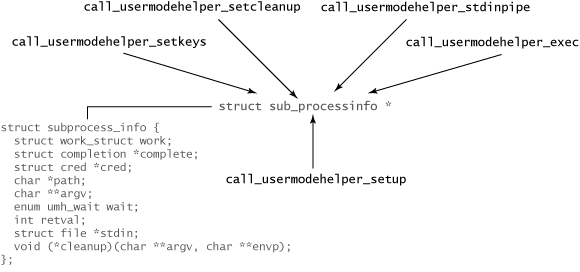
\includegraphics[scale = 0.6]{img/ris1.png}}
 			\label{ris:1}
 		\end{center}
 		\caption{Элементы интерфейса usermode-helper API.}
 	\end{figure}
 
 	Сокращенные функции из таблицы \ref{table2} внутри себя вызывают функцию \textit{call\_usermodehelper\_setup} и \textit{call\_usermodehelper\_exec}. Последние два вызова, указанные в таблице \ref{table2}, вызывают, соответственно, \textit{call\_usermodehelper\_setkeys} и \textit{call\_usermodehelper\_stdinpipe}. 
 	
 	
 	\subsection{Чтение из файла /proc/modules}
 	
 	Ниже приведен пример вывода информации из файла \textit{/proc/modules} с последующим объяснением значений.
 	
 	\begin{figure}[h!]
 		\begin{center}
 			{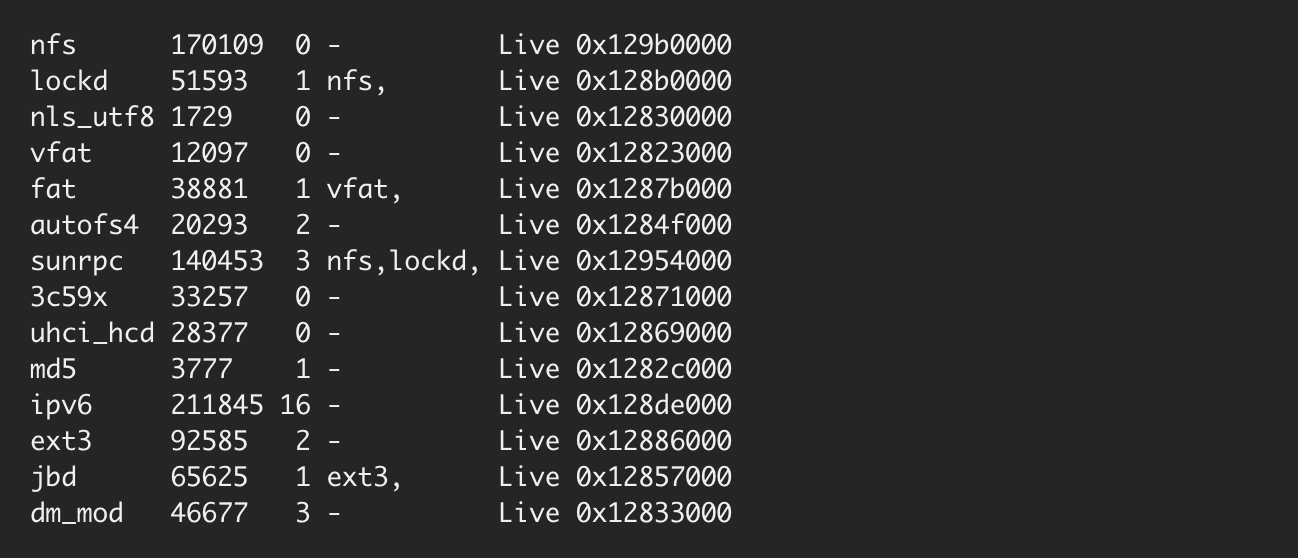
\includegraphics[scale = 0.6]{img/ris2.png}}
 			\label{ris:2}
 		\end{center}
 		\caption{Пример вывода \textit{/proc/modules}.}
 	\end{figure}
 
 	Где
 
 	\newpage
 
 	\begin{enumerate}
 		\item Имя модуля
 		\item Размер (в байтах) занимаемой модулем памяти
 		\item Количество загруженных экземпляров модуля. ноль — модуль выгружен
 		\item Список модулей, зависящих от данного
 		\item Текущее состояние модуля: Live — загружен, Loading — загружается и Unloading — выгружается
 		\item Текущее смещение в памяти программы linux, по которому загружен модуль
 	\end{enumerate}
 
 	\subsection{Схема алгоритма работы модуля ядра}
 	
 	Ниже приведена схема алгоритма работы модуля ядра.
 	
 	\begin{figure}[h!]
 		\begin{center}
 			{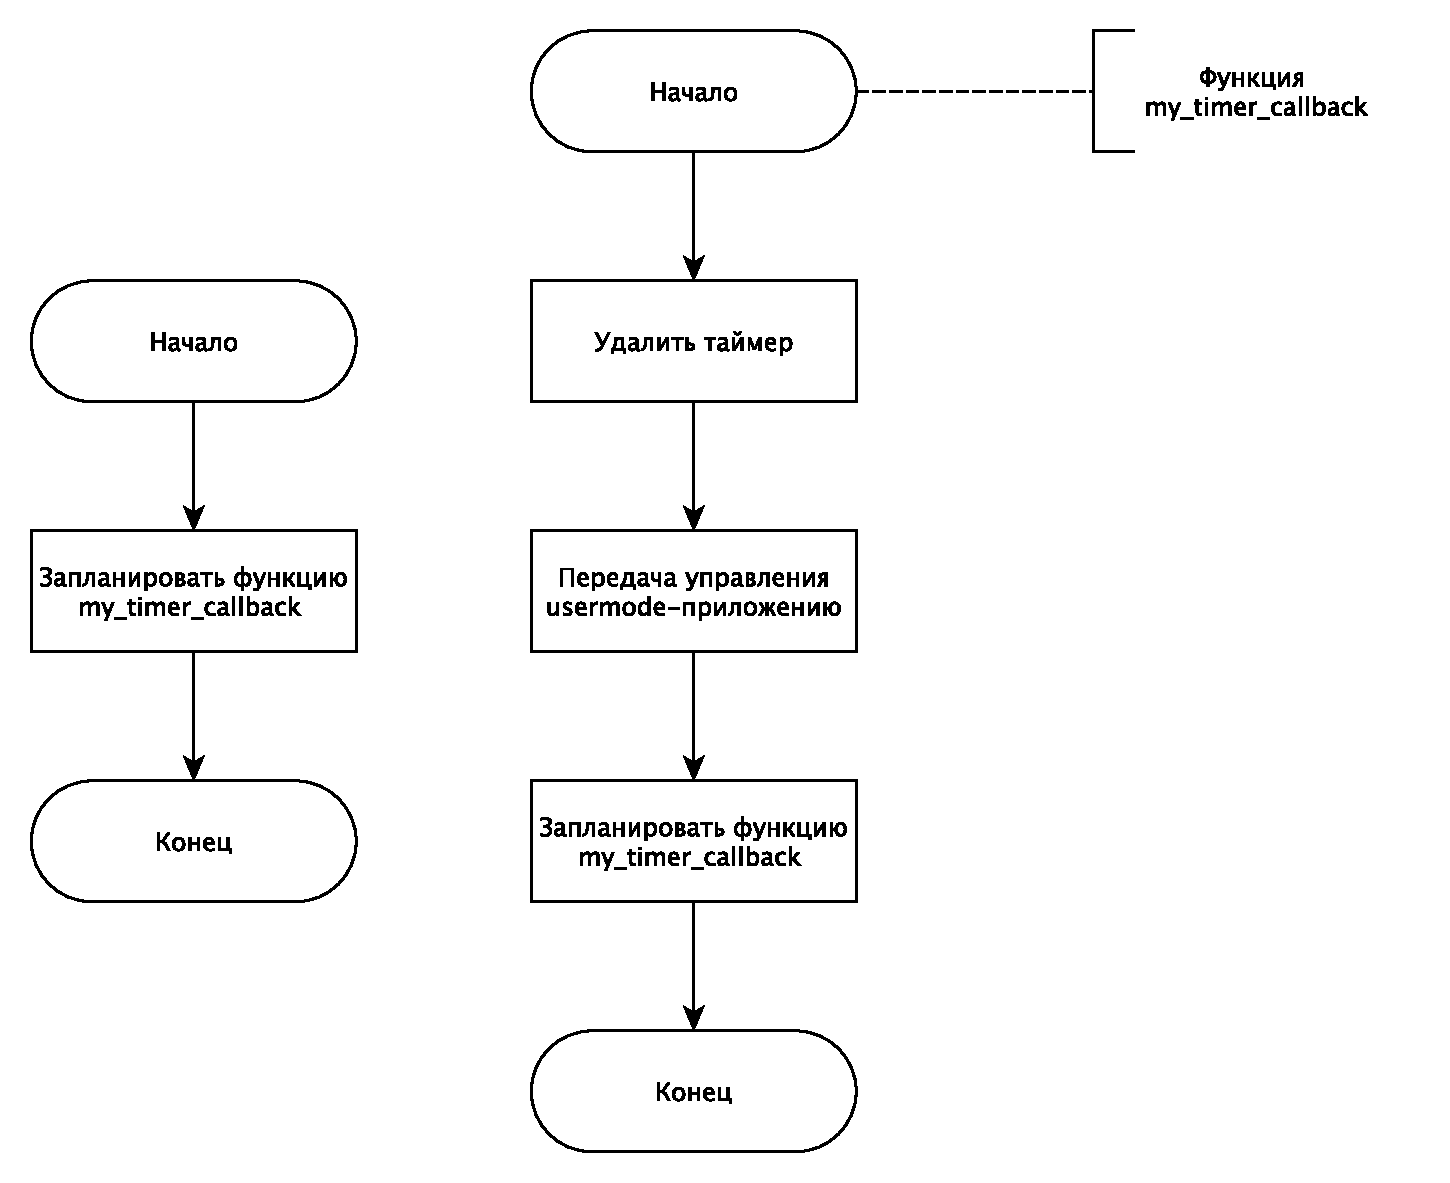
\includegraphics[scale = 0.6]{img/theme_kernel.pdf}}
 			\label{ris:theme_kernel}
 		\end{center}
 		\caption{Алгоритм работы модуля ядра.}
 	\end{figure}
 	
 	\subsection{Схема алгоритма работы usermode-приложения}
 	
 	Ниже приведена схема алгоритма работы приложения, работающего в пользовательском режиме.
 	
 	\begin{figure}[h!]
 		\begin{center}
 			{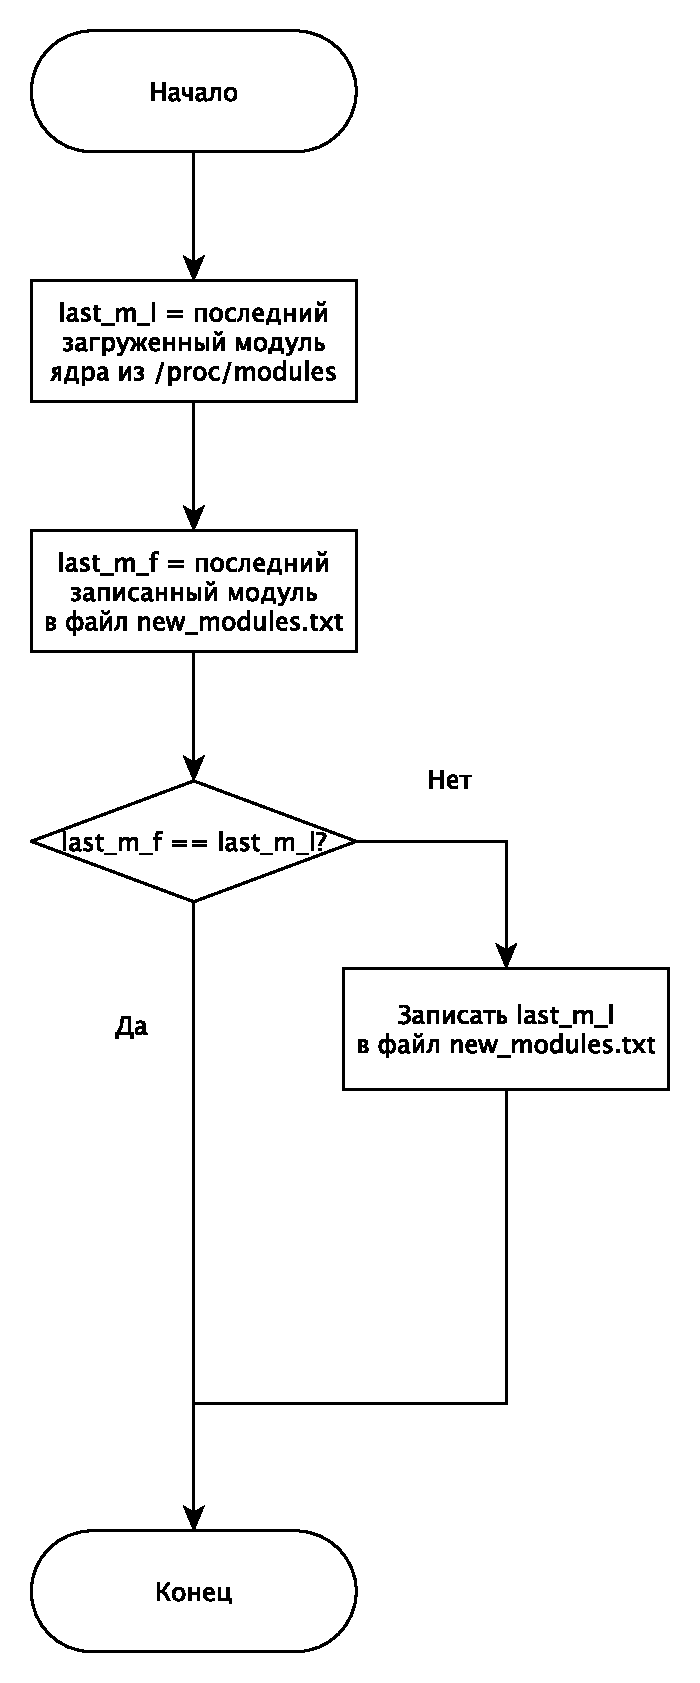
\includegraphics[scale = 0.6]{img/theme_usermode.pdf}}
 			\label{ris:theme_usermode}
 		\end{center}
 		\caption{Алгоритм работы usermode-приложения.}
 	\end{figure}
 
 	\newpage
 	
 	\subsection*{Выводы по конструкторскому разделу}
 	
 	Были проанализированы и изучены выбранные технологии для реализации поставленной задачи, в частности, API ядра Linux: API системных таймеров и usermode-helper API; а также структура файла /proc/modules.
 	
 	Были разработаны схемы алгоритмов работы обоих модулей программы.
 	
 	\newpage
 	
 	\section{Технологический раздел}
 	
 	\subsection{Выбор языка программирования}
 	
 	Для реализации загружаемого модуля был выбран язык С с использованием встроенного в ОС Linux компилятора GCC. Выбор языка основан на том, что исходный код ядра, предо­ ставляемый системой, написан на С, и использование другого языка программиро­ вания в данном случае было бы нецелесообразным.
 	
 	Для реализации приложения, работающего в пользовательском режиме, был выбран язык С++, поскольку он предоставляет удобный интерфейс для работы с файлами
 	
 	\subsection{Выбор среды разработки}
 	
 	Для написания программы, был выбран текстовый редактор Sublime text 3.
 	\begin{itemize}
 		\item Огромное количество плагинов, которые позволяют делать работу быстрее
 		\item Возможность гибкой настройки под себя
 		\item Много встроенных команд и комбинаций
 	\end{itemize}
 
 \newpage
 
 	\subsection{Модуль ядра}
 	
 	Ниже приведен листинг кода модуля ядра для данной работы.
 	
 	\begin{minted}{c}
#include <linux/init.h>
#include <linux/kernel.h>
#include <linux/module.h>
#include <linux/timer.h>
#include <linux/fs.h>
#include <linux/sched.h> 
#include <linux/uaccess.h>

void my_timer_callback(struct timer_list * my_timer);


#define TIMER 5000
#define USERMODE_PROGRAM \
"/home/ilalevuskin/Desktop/project/proc_modules"
#define FILE_NAME \
"/home/ilalevuskin/Desktop/project/new_modules.txt"

MODULE_LICENSE("GPL");
MODULE_AUTHOR("Levushkin Ilya");


static struct timer_list my_timer;

int init_timer(void)
{
	int ret;
	
	timer_setup(&my_timer, my_timer_callback, 0);
	
	ret = mod_timer(&my_timer, jiffies + \
	 msecs_to_jiffies(TIMER));
	if (ret)
	{
		printk("Error in mod_timer\n");
	}
	return ret;
}

void delete_timer(void)
{
	int ret;
	
	ret = del_timer(&my_timer);
	
	if (ret)
	{
		printk("The timer is still in use...\n");
	}
}

int print_new_load_proc_module_info(void)
{
	char *argv[] = {USERMODE_PROGRAM, FILE_NAME, NULL};
	static char *envp[] = {
	FILE_NAME,
	"TERM=linux",
	"PATH=/home/ilalevuskin/Desktop/project", NULL};
	call_usermodehelper(argv[0], argv, envp, UMH_NO_WAIT);
	return 0;
}


void my_timer_callback(struct timer_list * my_timer)
{
	delete_timer();
	print_new_load_proc_module_info();
	init_timer();
}

static int __init monitoring_init(void)
{
	int ret;
	printk("Monitoring module was installed\n");
	printk("Kernel modules info update (%d)ms (%ld)\n", \
	TIMER, jiffies);
	
	ret = init_timer();
	return ret;
}

static void __exit monitoring_exit(void)
{
	delete_timer();
	printk("Monitoring module uninstalled\n");
}

module_init(monitoring_init);
module_exit(monitoring_exit); 
 	\end{minted}
 	
 	\subsection{Приложение, работающее в режиме пользователя}
 	
 	Ниже приведен листинг кода приложения, работающего в режиме пользователя, для данной работы.
 	
 	\begin{minted}{c++}
#include <iostream>
#include <fstream>
#include <string>
#include <unistd.h>
#include <cstring>

using namespace std;

#define READ_PROC_ERR 1
#define WRITE_MODULE_ERR 2
#define READ_MODULE_ERR 3
#define OK 0


int get_last_module_to_kernel(string &buff)
{
	ifstream rfile;
	rfile.open("/proc/modules", fstream::in);
	getline(rfile, buff);
	rfile.close();
	return 0;
}

int get_last_added_module_to_kernel(string &res, \
string file_name)
{
	ifstream rfile;
	rfile.open(file_name.c_str(), fstream::in);
	
	if (!rfile)
	{
		return READ_MODULE_ERR;
	}
	
	string buf;
	while (getline(rfile, buf))
	{
		res = buf;
	}
	rfile.close();
	return 0;
}

int new_module_added(const char *last_module, \
const char* before_module)
{
	if (strcmp(last_module, before_module) != 0)
	{
		return 1;
	}
	return 0;
}

int write_added_module_in_file(string buff, string file_name)
{
	ofstream wfile;
	wfile.open(file_name.c_str(), ios::out | ios::app);
	
	if (!wfile)
	{
		return WRITE_MODULE_ERR;
	}
	
	wfile << buff << endl;
	
	wfile.close();
	return OK;
}

int main(int argc, char *argv[])
{
string buff_1, buff_2;
if (argv[1])
{
	string file_name = argv[1];
	if (get_last_module_to_kernel(buff_1))
	{
		cerr << "Cannot read /proc/modules" \
		<< endl;
		return READ_PROC_ERR;
	}
	if (get_last_added_module_to_kernel(buff_2, file_name))
	{
		cerr << "Cannot read file " \
		<< file_name.c_str() << endl;
		return READ_MODULE_ERR;
	}
	if (new_module_added(buff_1.c_str(), buff_2.c_str()))
	{
		if (write_added_module_in_file(buff_1, \
		file_name))
		{
			cerr << "Cannot write in file " \
			<< file_name.c_str() << endl;
			return WRITE_MODULE_ERR;
		}
	}
	return OK;
}
else
{
	cerr << "No arguments were transfered" << endl;
}
}
 	\end{minted}
 	
 	
 	\subsection*{Выводы по технологическому разделу}
 	
 	Были даны обоснования по выбору языка программирования и среды разработки, приведены листинги кода двух модулей программного обеспечения.
 	
 	
 	\newpage
 	\section*{Заключение}
 	\addcontentsline{toc}{section}{Заключение}
 	
 	В результате выполнения данной курсовой работы были изучены основные способы планирования исполнения задач в ядре Linux.
 	
 	Была исследована структура файловой системы proc.
 	
 	Разработано программное обеспечение, позволяющее осуществлять вывод информации о загруженных модулях ядра Linux.
 	
 	Реализован модуль ядра, позволяющий вызывать через заданные промежутки времени приложение, работающее в пользовательском режиме.
 	
 	Реализовано приложение, выводящее в конец файла информацию о последнем загруженном модуле ядра в систему.
 	
 	
 	
 	
 	\newpage
 	
 	\addcontentsline{toc}{section}{Список используемой литературы}
 	\begin{thebibliography}{5}
 		\bibitem{usermode}
 		Вызов приложений, работающих в пользовательском пространстве, из ядра системы [Электронный ресурс]. – Режим доступа: 
 		http://rus-linux.net/nlib.php?name=/MyLDP/kernel/api/kernelapi1.html, 
 		свободный – (02.12.2020)
 		\bibitem{tsirulik}
 		Модули Linux ядра, Олег Цилюрик [Электронный ресурс]. – Режим доступа: 
 		http://rus-linux.net/MyLDP/BOOKS/Moduli-yadra-Linux/KERN-modul-4.95.pdf, 
 		свободный – (02.12.2020)
 		\bibitem{proc}
 		Файловая система proc [Электронный ресурс]. – Режим доступа: 
 		https://www.opennet.ru/man.shtml?topic=proc\&category=5\&russian=0, 
 		свободный – (02.12.2020)
 		\bibitem{proc2}
 		ФАЙЛОВАЯ СИСТЕМА PROC В LINUX [Электронный ресурс]. – Режим доступа: 
 		https://losst.ru/fajlovaya-sistema-proc-v-linux\#/proc/modules, 
 		свободный – (02.12.2020)
 		\bibitem{time}
 		Течение времени в ядре Linux [Электронный ресурс]. – Режим доступа: 
 		http://knzsoft.ru/ldd2-ch6/\#t3, 
 		свободный – (02.12.2020)
 	\end{thebibliography}
 	
 \end{document}